\documentclass[12pt,letterpaper]{article}
\usepackage[utf8]{inputenc}
\usepackage{amsmath}
\usepackage{amssymb}
\usepackage{graphicx}
\usepackage{natbib}
\usepackage{pgfplots}  % For generating graphs within LaTeX
\usepackage{hyperref}
\usepackage{setspace}

\title{Note: the market for elite status-initial draft}
\author{Joao Faria and Michael Ryall}
\date{\today}

\begin{document}
	
	\maketitle

	
%	\begin{abstract}
%		Your abstract goes here...
%	\end{abstract}
	
	\onehalfspacing
	
	\section{Introduction}
	There are two questions that we are each working on. 
	The first is, given certain assumptions about people's quest for elite status and its effect on productivity, what dynamic equilibria look like.
	The second is how the ``inefficient'' equilibria that appear in the answer to question \#1 can survive in a free market; i.e., why don't the forces of competition eliminate them.
	The first question can be answered using a partial equilibrium approach, which is what our first model is.
	The second requires a complete GE model, which is what I hope to outline in this note.
	
	What I am guessing is that we will want toexplore both approaches (.e.g., by working through numerical examples), then work toward converging the approaches by tweaking up the models so that they are as closely related as possible. 
	This note is an initial exploration of the full GE approach.
%	


%	\begin{figure}[ht]
%		\centering
%		\begin{tikzpicture}
%			\begin{axis}
%				% Graph generated within LaTeX goes here...
%			\end{axis}
%		\end{tikzpicture}
%		\caption{Caption for your generated graph.}
%		\label{fig:latexgraph}
%	\end{figure}
	
	\section{General model}
	I will approach this in two steps. 
	First, I will map Ellickson et al. (2007) to our  general case (i.e., as a special case of the Ellickson et al. general model but as the general case of concern to us).
	Second, I will work through some numerical examples.
	
	\subsection{Groups and memberships}
	There are two divisible, publicly traded private goods, $y_1$ and $y_2$, which we can think of as money and a consumption good. Then, $y=(y_1,y_2)\in\mathbb{R}^2$.
	
	There are four group types: i) the group of the socially elite; ii) \textit{Elite degree mills}; iii) \textit{Serious universities}; and iv) \textit{firms}.
	Group types are defined by their membership characteristics and organizational characteristics.
	
	Let $\Omega$ and $\Gamma$ be finite sets of \textit{membership characteristics} and \textit{organizational characteristics}, respectively. 
	A \textit{group type} is a triple $(\pi,\gamma,y)$ consisting of a \textit{profile} $\pi:\Omega\rightarrow\{0,1,\ldots\}$, an \textit{organizational characteristic} $\gamma\in\Gamma$, and an \textit{input-output vector} $y\in\mathbb{R}^2$.
	There will be a finite set of possible group types $\mathcal{G}=\{(\pi,\gamma,y)\}$.
	
	For $\omega\in \Omega$, $\pi(\omega)$ represents the number of members with the membership characteristic $\omega$ that the group is required to have, so $|\pi|=\sum_{\omega\in\Omega}\pi(\omega)$ is the total number of members that the group is required to have.\footnote
		{
		``A membership characteristic is anything that matters to the individual who comprise a group or to the activity in which the group is engaged. In particular, a membership characteristic can encompass personal qualitites qualities (intelligence, appear- ance, personality, etc.), roles within the group (teacher, student, supervisor, skilled laborer, unskilled laborer, etc.) and skills (singing, dancing, language, etc.). Formally, all membership characteristics are acquired; membership characteristics that are innate (height for instance) are encompassed in our specification of consumption sets below. [In our earlier paper, we insisted that membership characteristics be innate and fixed.] Importantly, membership characteristics are observable and contractible. We emphasize that $\Omega$ is simply an abstract finite set. In particular, $\Omega$ is not a vector space and need not have any linear structure.''
	}
	
	In this case, it seems that what we need is fairly straightforward in terms of groups and requisite membership characteristics:
	\begin{enumerate}
		\item \textit{Elite degree mills} take in students, no membership characteristics required, and confer elite status (but have no effect on managerial skills). 
		\item \textit{Serious universities} also take in anyone. These confer actual managerial skill.
		\item The \textit{socially elite} requires having completed education in an Elite degree mill.
		\item \textit{Firms} will require managers and laborers. Managers are those who graduate from a university. Those from serious universities are more productive. 
	\end{enumerate}
	It would also be interesting to introduce high and low quality faculty and see where they migrate, but not for now.\footnote
	{ 
		``An organizational characteristic might be anything that matters to the potential member of a group apart from the characteristics of the members in the group and the input-output vector. In particular, an organizational characteristic can encompass the activity within the group (that is, the process used to produce output), the organizational hierarchy within the group, and the duties of each potential member of the group.''
	}
	Clearly, elites will want to be with other elites in firms -- this is a key part of the model. 
	We might even assume that laborers prefer \textit{not} to work in firms run by elites.
	But, these are characteristics of firm members.
	So, the only things that seem to fit the requirements for organizational characteristic are the university processes (degree mills or actual learning centers).
	These are organizational characteristics because they are not determined by member characteristics or the input-output vector.
	Colleges produce ``education'' (of one form or the other) and take tuition.
	[Not clear if education is also a publicly traded good.]
	Firms, of course, produce products and pay wages.
	
	A membership is a pair $m=(\omega,(\pi,\gamma,y))$ such that $(\pi,\gamma,y)\in\mathcal{G}$ and $\pi(\omega)\ge 1$. Let $\mathcal{M}$ be the finite set of group memberships. Agents choose a bundle of memberships, referred to as a \textit{list}, which is a function $l:\mathcal{M}\rightarrow\{0,1,\ldots\}$; $l(m)$ specifies the number of memberships of type $m=(\omega,(\pi,\gamma,y))$.
	The set of lists is denoted \textbf{Lists}.
	
	\subsection{Agents}
	The set of agents is a nonatomic finite measure space $(A,\mathcal{F},\lambda)$: $A$ is a set, $\mathcal{F}$ a $\sigma$-algebra of subsets of $A$, and $\lambda$ is a non-atomic measure on $\mathcal{F}$ with $\lambda(A)<\infty$.
	A complete description of $a\in A$ consists of a \textit{consumption set}, an \textit{endowment vector} of private goods, and a \textit{utility function}. 
	
	\subsubsection{Consumption sets}
	Agent $a$'s consumption set $X_a$ specifies the feasible pairs of bundles of private goods and lists of membership that the agent may choose.
	Assume the following:
	\begin{enumerate}
		\item $X_a\subset\mathbb{R}^2_+\times\textbf{Lists}$,
		\item If $(x_a,\mu_a)\in X_a$ and $x^\prime_a\ge x_a$ then $(x^\prime_a,\mu_a)\in X_a$,
		\item There exists $M>0$ such that for all $a\in A$ and all $(x_a,\mu_a)\in X_a$
		\[
		\sum_{m\in\mathcal{M}}\mu_a(m)\le M.
		\]
	\end{enumerate}
	The first condition says private good consumption must be nonnegative. 
	The second says increased consumption of private goods is always possible.
	The last says that the number of memberships each agent can choose is bounded.
	In particular, for each agent $a\in A$, the set
	\[
	\textbf{Lists}_a\equiv\{\mu_a\in\textbf{Lists}|\exists x_a\in \mathbb{R}^2_+ \text{ s.t. }(x_a,\mu_a)\in X_a\}
	\]
	is finite.\footnote
	{
		``A choice $(x_a,\mu_a)$ is in $X_a$ if it is possible for agent $a$ to consume the bundle of private goods $x_a$ and fulfill the requirements of the memberships specified by $\mu_a$.
		The consumption set $X_a$ encodes restrictions on the choices that $a$ can make with respect to both private goods and memberships.''
	}
	
	In our setting, elite education is required for being part of the elite group.
	In addition, any education is required to be in the managerial class.
	Let $f,f^\ast,s,s^\ast\in\mathcal{G}$ be a firm,  an elite firm, a serious school of higher education, and an elite degree mill, respectively.
	Then, $(\omega,f)$ requires that $\omega$ be ``holds a college degree of either kind.''
	
	Thus, we insist that if $(\mu_a,f)\in X_a$ and $\mu_a(\omega,f)>0$, then $\mu_a(\omega^\prime,s)>0$ or  $\mu_a(\omega^\prime,s^\ast)>0$.
	Similarly, if $(\mu_a,f^\ast)\in X_a$ and $\mu_a(\omega,f^\ast)>0$, then $\mu_a(\omega^\prime,s^\ast)>0$.
	(It is for this reason that we cannot assume $X_a=\mathbb{R}^2_+\times\textbf{Lists}$.)\footnote
	{
		``Much of the flexibility of our model arises from the fact that an agent can choose (memberships with) different characteristics in different groups. In particular, we allow an agent to fill different roles in different groups — to provide barber services in one group and receive them in another. The possibility of filling different roles in different groups is essential to the way we model the acquisition of skills, which will typically be acquired in one venue and applied in another. Of course, the acquisition of skills usually precedes their application; we incorporate the temporal element by viewing the date or time period as part of the description of a group, just as traditional general equilibrium theory frequently views the date or time period as part of the description of a commodity.''
	}
	This suggests that part of the descriptions of schools include a date $t$ and of firms a date $t+1$.
	
	\subsubsection{Endowments}
	Agent $a$'s \textit{endowment} is $(e_a,0)\in X_a$. 
	Agents are endowed with private goods but not with group memberships.

	\subsubsection{Utility functions}
	Agent $a$'s \textit{utility function} is $u_a:X_a\rightarrow \mathbb{R}$ is defined over private goods conumptions and lists of group membership.
	Assume, for each $\mu_a\in\textbf{ Lists}$,
	\[
	 u_a(\cdot,\mu_a):\{x_a|(x_a,\mu_a)\in X_a\}\rightarrow \mathbb{R}
	 \]
	 is continuous and strictly monotone; i.e., utility is strictly increasing in consumption of private goods.
	 No assumptions are made about the way in which utility depends on the choice of group memberships.
	 
	 \subsection{Economies}
	 An \textit{economy} $\mathcal{E}$ is a mapping $a\mapsto(X_a,e_a,u_a)$ for which:
	 \begin{itemize}
	 	\item The consumption set correspondence $a\mapsto X_a$ is a measurable correspondence.
	 	\item The endowment mapping $a\mapsto e_a$ is an integrable function.
	 	\item The utlity mapping $(a,x,l)\mapsto u_a(x,l)$ is a jointly measurable function of its arguments.
	 \end{itemize}
	 We may  that agents begin only with an endowment of money (e.g., $Y$ in our dynamic model).
	 
	 \subsection{States}
	 A \textit{state} of an economy is a measurable mapping
	 \[
	 (x,\mu):A\rightarrow \mathbb{R}^2\times\mathbb{R}^\mathcal{M}.
	 \]
	A state specifies choices of private goods and group memberships.
	Feasibility of a state of the economy is defined as feasibility of the consumption and productions plans and consistent matching of agents.
	In our case, we will require that there be some fixed fraction of managers to workers for the set of firms (i.e.g, because the set of agents is a continuum).
	Of course, we can have different types of firm and these can have production technologies that require a different ratio of managers to workers.
	
	To formalize this idea, define the \textit{membership vector} $\bar{\mu}\in \mathbb{R}^\mathcal{M}$.
	An aggregate membership vector $\bar{\mu}$ is consistent if for every group type $(\pi,\gamma,y)\in\mathcal{G}$, there is a real number $\alpha(\pi,\gamma,y)$,
	\[
	\bar{\mu}(\omega,(\pi,\gamma,y))=\alpha(\pi,\gamma,y)\pi(\omega)
	\]
	for each $\omega\in\Omega$. Given a measurable set $B\subset A$ and a measurable choice function $\mu:B\rightarrow\textbf{Lists}$, we say that $\mu$ is \textit{consistent for} $B$ if the aggregate membership vector $\int_B\mu_ad\lambda(a)$ is consistent.
	
	Then, $(x,\mu)$ is \textit{feasible for} the measurable subset $B\subset A$ if
	\begin{enumerate}
		\item \textbf{Individual feasibility}:  $(x_a,\mu_a)\in X_a\text{ for each } a\in B$
		 \item \textbf{Material balance}: 
		 \[
		 \int_B x_a d\lambda(a)\le \int_B e_a d\lambda(a) + 
		 \left[
		 \sum_{(\omega,(\pi,\gamma,y))} \mu_a(\omega,(\pi,\gamma,y))\frac{y}{|\pi|}
		 \right]d\lambda(a).
		 \]
		 \item \textbf{Consistency}: $\int_B\mu_a d\lambda(a)$ is consistent for $B$.
	\end{enumerate}
	Item 1 says $(x,\mu)$ is feasible for $B$ if individuals in $B$ choose profiles in their consumption sets, private consumption does not exceed the sum of endowments, and net production and agents are matched consistently.
	The state $(x,\mu)$ is \textit{feasible} if this condition applies to $A$.
	If $(x,\mu)$ is  a state of  the economy, $m=(\omega,g)$ is a membership and $\mu_a(m)>0$, $a$ is said to \textit{choose} the membership $m$.
	
	If $(x\mu)$ is consistent for $B$ and $\int_B \mu_a d\lambda(a)=\alpha(\pi,\gamma,y)\pi(\omega)$ for each $\omega\in\Omega$, then material balance is equivalent to the assertion that 
	\[
	\int_B x_a d\lambda(a)\le \int_B e_a d\lambda(a) + 
	\sum_{(\pi,\gamma,y)\in\mathcal{G}} \alpha(\pi,\gamma,y)y.
	\]
	Members of a group only consider the membership characteristics of other members and their identities
	Therefore, it is not necessary to identify the agents belonging to each group by individual.
	
	\subsection{Group equilibrium}
	Both private goods and group memberships are priced, so prices $(p,q)\in\mathbb{R}^2\times\mathbb{R}^\mathcal{M}$.
	In other words, $p$ is the vector of prices for private goods and $q$ is the vector of prices for group memberships.\footnote 
	{
		``Because utility functions are assumed monotone in private goods, private goods prices will be positive in equilibrium, but prices of group memberships may be positive, negative or zero. Because a membership specifies both a group type and a membership characteristic, membership prices depend both on the group type and the membership characteristic.''
	}
	
	A group equilibrium consists of prices $(p,q)\in\mathbb{R}^2\times\mathbb{R}^\mathcal{M}$, with $p\ne 0$ and a feasible state $(x,\mu)$ such that 
	\begin{enumerate}
		\item \textbf{Budget balance for group types}: For each $(\pi,\gamma,y)\in\mathcal{G}$:
		\[
		\sum_{\omega\in\Omega}\pi(\omega)q(\omega,(\pi,\gamma,y))+p\cdot y=0.
		\]
		\item \textbf{Budget feasiblity for agents}: For almost all $a\in A$,
		\[
		(p,q)\cdot(x_a,\mu_a)\le p\cdot e_a.
		\]
		\item \textbf{Optimization by agents}: For almost all $a\in A$,
		\[
		(x^\prime_a,\mu^\prime_a)\text{ and } u_a(x_a,\mu_a)\Rightarrow (p,q)\cdot	(x^\prime_a,\mu^\prime_a)>p\cdot e_a.
		\]		
	\end{enumerate}
	In other words, in equilibrium the sum of membership prices in a given group type just balances the value of the input-output vector and individuals optimize subject to their budget constraints.
	
	\section{Details for our case}
	
	\subsection{Agents}
	Assume a continuum of agents $A$. 
	All agents are ex-ante identical. 
	Each has endowment $e=(k,0)\in\mathbb{R}^2_+$, where we can think of $k$ as the (per capita) wealth of the economy.
	The first component is the quantity of input (a resource good) and the second is the quantity of output (a consumption good).
	
	\subsection{Groups}
	The indexed set of membership characteristics is  $\Omega=\{\omega_1,\ldots,\omega_4\}$ where  $\omega_1=S$ represents a student at a university, $\omega_2=M$ a manager, $\omega_3=EM$ an elite manager, and $\omega_4=L$ a laborer.
	
	There are four group types. 
	Serious schools are type $g_1=((S),s,y_s)$, in which the only member role is $\pi_s=(S)$, a student, and $y_s=(-r,0)$ because the university requires basic inputs of $r\ge 0$ to educate an individual student.\footnote
	{
		Note that writing $\pi_s=(S)$ is another abuse of notation since $\pi$ is a profile; i.e., $\pi_s=(1,0,0,0)$ is the technically correct, but more cumbersome, representation.
	}
	Similarly, $g_2=((S),s^\ast,y_{s^\ast})$ with  $y_{s^\ast}=(- \tau  r,0)$, where $\tau\ge 1$ is a parameter that accounts for the possibility that elite universities consume more resources than serious universities (on such things as beautiful facilities in geographically expensive areas, research faculty who do relatively little teaching, etc).
	
	Firms are also of two types, those run by well-trained managers and those run by elite managers.
	Let $g_3=((M,2L),f,y_f)$, which indicates that one manager and two laborers are required to staff a firm.
	Then $y_f=(-y_{f1},y_{f2})$ is the competent firm's production function in which $y_{f1}$ units of the input good are required to produce$y_{f2}$ units of the output good.
	Specifically, assume $y_f=(-c,\phi)$ where $\phi$ is the basic level of output common to both firm types.
	
	Similarly, there is a type of firm run by elite managers,   $g_4=((EM,2L),f,y_{f^\ast})$, in which one manager and two laborers are required and $y_{f^\ast}=(- \beta c,\alpha\phi)$ where $\beta\ge 1$ is a multiplier that accounts for input productivity differentials between the firm types (e.g, $\beta>1$ would reflect the fact that because elite universities do not actually teach anything, elite managers run their businesses less efficiently, such as by engaging in  signaling elite status by wasting firm resources in public displays of elite solidarity).
	Similarly,   $\alpha\ge 0$ is a multiplier that allows us to account for an output productivity differential between firms
	
	The set of possible group memberships, $\mathcal{M}$, contains the following elements:
	\begin{align*}
		&m_1=(S,g_1),m_2=(S,g_2),\\
		&m_{3.1}=(M,g_3),m_{3.2}=(L,g_3),\\
		&m_{4.1}=(EM,g_4),m_{4.2}=(L,g_4).
		.
	\end{align*}
	We assume that no agent can attend more than one university or work for more than one firm as either a manager or a laborer.
	Managers are those that attended a serious university and elite managers must have attended an elite university. 
	Thus, for all individuals,
	\begin{align*}
		\textbf{Lists}=\Big\{l|
		&l(m_1)+l(m_2)\le1,\\
		&l(m_{3.1})+l(m_{3.2})+l(m_{4.1})+l(m_{4.2})\le1\\
		&l(m_{3.1})\le l(m_1),\\
		&l(m_{4.1})\le l(m_2)\Big\}.
	\end{align*}
	
	\subsection{Utility}
	Since all agents are ex-anti identical, there is only one utility function.
	Individuals can make the following vocational choices in order of preference for a given level of consumption:
	\begin{enumerate}
		\item No memberships: $l$ such that, for all $m\in\mathcal{M}$, $l(m)=0$,
		\item Become an elite manager: $l(m_2)=l(m_{4.1})=1$,
		\item Become a manager: $l(m_1)=l(m_{3.1})=1$,
		\item Become an uneducated laborer managed by a competent manager: $l(m_{3.2})=1$, $l(m_1)=l(m_2)=0$,
		\item Become an uneducated laborer managed by an elite manager: $l(m_{4.2})=1$, $l(m_1)=l(m_2)=0$.
	\end{enumerate}
	Denote these \textit{choices} as $C_1,\ldots,C_5$.
	There are two other feasible choices not listed here. 
	One is to go to school then work for no firm. 
	The other is to go to school and to work as a laborer. 
	The first will be strictly dominated by Choice (1) and the second will be strictly dominated by (2), both because going to school and not becoming a manager of some kind will add disutility without any additional payoff (as assumed below).
	The implicit assumption is that laborers don't like working for no-talent elites. 
	
	Let utility be given by:
	\[
	u(y,l) = \begin{cases}
		D_1h(y_1,y_2)\text{ if choice (1)}  \\
		D_2h(y_1,y_2)\text{ if choice (2)} \\
		D_3h(y_1,y_2)\text{ if choice (3)} \\
		D_4h(y_1,y_2)\text{ if choice (4)} \\
		D_5h(y_1,y_2)\text{ if choice (5)} \\
	\end{cases}
	\]
	where $h$ is the utility an agent receives from a consumption bundle without having gone to university or having had to work.
	Assume $h_{y_j}>0$, $h_{y_iy_j}>0$ for $i\ne j$, and $h_{y_j^2}<0$.
	Consistent with our story, assume $D_1>\ldots> D_5$.
	
	For now, assume $h(y_1,y_2)=\sqrt{y_1,y_2}$ (we can write the analysis in terms of the conditions for a more general $h$ later).
	To keep things tractible (and to track the example in Ellickson et al. as closely as possible for now), let the $D_i$'s be in decreasing multiples of two: $D_1=32,D_2=16,\ldots, D_5=2$.
	
	\subsection{Equilibrium}
	
	The private goods and memberships are all priced.
	Let $p(p_1,p_2)$ be the prices for the input and output goods and $q=(q_1,q_2,q_{3.1},q_{3.2},q_{4.1},q_{4.2})$ be the prices for the group memberships.
	Normalize so that $p_1=1$.
	Since agents are ex-ante identical, choices can be described by the fractions of agents, $\sigma_0,\sigma_1,\sigma_2$, making choices to either engage in 100\% leisure, work for the elite firm, or work for the productive firm, respectively.
	Keep in mind that within $\sigma_1$ and $\sigma_2$, in any equilibrium $\frac{1}{3}$ must be managers and $\frac{2}{3}$ laborers.
	Of course, $1=\sigma_0+\sigma_1+\sigma_2$.
	
	The indirect utilities are defined in terms of $p$, $q$, $k$, and the agent's vocational choice, $C_j$. 
	These are defined below (where $p_1=1$ and ``$:=$'' means ``is defined as''):
	\[
	v(p,q,k,C_j) = \begin{cases}
		V(1):=16k/\sqrt{p_2}\text{ if }j=1\\
		V(2):=8(k-q_2-q_{4.1})/\sqrt{p_2}\text{ if }j=2\\
		V(3):=4(k-q_1-q_{3.1})/\sqrt{p_2}\text{ if }j=3\\
		V(4):=2(k-q_{3.2})/\sqrt{p_2}\text{ if }j=4\\
		V(5):=(k-q_{4.2})/\sqrt{p_2}\text{ if }j=5
	\end{cases}
	\]
	These follow from optimizing given the price, endowment and choice parameters (easy to show).
	There are several budget balance conditions for the various groups.
	For the serious and elite universities, respectively, we have
	\begin{align}
		q_1-r&=0,\label{Eq:u-balance1}\\
		q_2-\tau r&=0,\label{Eq:u-balance2}
	\end{align}
	Where $q_1$ and $q2$ represent tuition payments by students.
	For the serious and elite firms, respectively, the budget balance conditions are:
	\begin{align}
		q_{3.1}+2q_{3.2}+p_2\alpha\phi-c&=0,\label{Eq:f-balance1}\\
		q_{4.1}+2q_{4.2}+p_2\phi-\beta c&=0.\label{Eq:f-balance2}
	\end{align}
	It can be shown that the market clearing condition for the input good requires\footnote
	{
		These are derived while solving for the indirect utilities above. I have the calculations on paper and can put the them in an appendix later.
	}
	\begin{align*}
	k=\sigma_0\left[\frac{k}{2}\right] 
	&+ \sigma_1
	\left[
		\frac{2}{3}\left(\frac{k-q_{4.2}}{2}\right)
		+\frac{1}{3}\left(\frac{k-q_2-q_{4.1}}{2}\right)
	\right]\\
	&+ \sigma_2
	\left[
		\frac{2}{3}\left(\frac{k-q_{3.2}}{2}\right)
		+\frac{1}{3}\left(\frac{k-q_1-q_{3.1}}{2}\right)
	\right]\\
	&+
	\sigma_1(\tau r+\beta c) + \sigma_2(r+c),
	\end{align*}
	where the first two lines are per capita demand by consumers and the last line accounts for inputs required to run schools and firms.
	Recall that
	\begin{align}\label{eq:sumsigmas}
		\sigma_0+\sigma_1+\sigma_2=1
	\end{align} 
	
	Using \eqref{Eq:u-balance1} through \eqref{eq:sumsigmas}, the market clearing equation simplifies to
	
	\begin{align}
		3k&=\sigma_1
		\Big(
		\tau r + \beta c + p_2\alpha\phi
		\Big) 
		+\sigma_2
		\Big(
		r + c + p_2\phi
		\Big)\label{MktClear}
	\end{align}
	
	Consider an equilibrium in which $\sigma_1,\sigma_2,\sigma_3>0$. 
	Since all the agents are ex-ante equivalent, choices $V(1)$ through $V(5)$ must provide equal utility.
	Therefore, the prices for group memberships are as follows:
	\begin{align*}
	\phantom{====}	q_1&=r&&\text{ tuition for serious university}\\
	\phantom{====}	q_2&=\tau r&&\text{ tuition for elite university}\\
	\phantom{====}	q_{4.1}&=-\tau r&&\text{ wage for elite manager}\\
	\phantom{====}	q_{3.1}&=-(k+r)&&\text{ wage for competent manager}\\
	\phantom{====}	q_{4.2}&=-15k&&\text{ wage for laborer managed by elite}\\
	\phantom{====}	q_{3.2}&=-3k&&\text{ wage for laborer managed by competent}.		
	\end{align*}
	Here are some things to note. 
	Universities get reimbursed for their tuition.
	Managers pay for this, which is reflected in their compensation. 
	Notice that elite managers are so happy to be in the elite that elite firms only reimburse them for their tuition and nothing more (given the price of elite university educations, this doesn't seem unrealistic).
	
	We assume that elite universities signal their elite status by essentially burning resources (e.g., hiring world-famous researchers who, as it turns out, don't actually teach anything but ensuring $\tau>1$).
	Since tuition reimbursement shows up in the compensation of managers, this model posits that when elite manager compensation is significantly higher than that of competent managers, the gain is entirely due to their need to be reimbursed for their expensive elite education.
	This implies that elite schools are pulling in tons of tuition \ldots to compensate expensive professors who don't produce anything that is actually useful! 
	
	What's funny is that, given how much they hate working for the elite, laborers working for elite (e.g., woke) firms have to be paid a lot more than their counterparts working in normal companies.
	
	With these prices in hand, we can compute the price of $p_2$ from the budget-balance conditions \eqref{Eq:f-balance1} and \eqref{Eq:f-balance2}.
	\begin{align}
		p_2=\left(6k+r+c\right)/\phi
		=\left(30k+\tau r+\beta c\right)/(\alpha\phi).\label{PriceOf2}
	\end{align}
	
	This allows us to think, for example, about how equilibrium depends upon the output capability of elite firms and the wealth of society when the other parameters are fixed.
	Writing the $\alpha$ that satisfies the preceding equations as a function of $k$,
	\begin{align}
		\alpha(k):=\frac{30k+\beta c+\tau r}{7k+c+r}.
	\end{align}
	Note that   $\alpha(k)>1$ for all feasible parameter configurations.
	Keep in mind that these are the parameter values for which equilibria exist such that positive shares of the population engage in all vocational choices.
	
	Finally, we wish to solve for $\sigma_1$ in terms of $\sigma_2$ in terms of $\sigma_0$. From market clearing \eqref{MktClear} and the equilibrium prices,	
	\begin{align}
		\sigma_1&=
		\frac{3k-(1-\sigma_0)(1-\sigma_0)(2r + 2c +7k)}
		{23k + 2r(\tau-1) + 2c(\beta-1) +23k}\label{Example Sigma1}.
	\end{align}
	and
	\begin{align}
		\sigma_2&=
		\frac{3k-(1-\sigma_0)(2r\tau + 2c\beta +30k)}
		{-23k + 2r(1-\tau) + 2c(1-\beta)}.\label{Example Sigma2}			
	\end{align} 
	
	
	\section{Numerical example}
	Let us construct a tractable numerical example by which to examine the relationship between societal wealth, $k$, productive inefficiency, $\beta$, and the proportions of people who sort in to each membership role, $\sigma_1,\sigma_2,\sigma_3$.
	Assume parameters take the following values:
		\begin{align*}
		\phantom{====}	r&=1&&\text{ cost to operate effective universities}\\
		\phantom{====}	\tau&=2&&\text{ tuition multiplier for elite universities is irrelevant}\\
		\phantom{====}	c&=1&&\text{ resource us for productive firms}\\
		\phantom{====}	\phi&=6&&\text{ output for productive firms}\\
		\phantom{====}	\beta&=2&&\text{ resource useage multiplier for elite firms}\\
		\phantom{====}	\alpha&=?&&\text{ output multiplier for elite firms}		
	\end{align*}
	
	This results in the following function  
	\begin{align}
		\beta(k)=\frac{30k+4}{7k+4}.\label{alpha parameterized}
	\end{align}
	This function gives the parameter values $(\alpha,k)$ for which equilibria exist such that $\sigma_0,\sigma_1,\sigma_2>0$. 
	
	\begin{figure}[h]
		\centering
		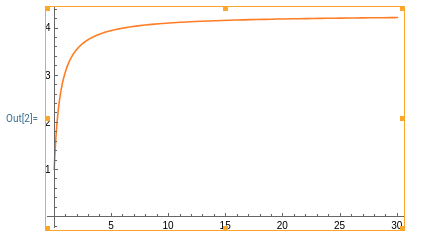
\includegraphics[width=1.0\textwidth]{Alpha of k}
		\caption{Graph of $\alpha(k)$ with $k$ on the $x$-axis. These are parameter values for $(x,\alpha)$ such that equilibria exist in which all vocations are engaged in equilibrium. A complete phase diagram will describe what happens in the economy on either side of the line. That can be done next.}
		\label{fig:my_label}
	\end{figure}
	
	
	
	
	These equilibria are characterized by choosing  
	\begin{align}
		\sigma_0\in\left[\frac{4k+4}{7k+4},\frac{27k+8}{30k+8}\right].\label{Paramter Constraints 2}
	\end{align}
	Notice that if there is no endowment, $k=0$ and everyone enjoys their ``leisure''.
	
	
	
	
	
%	\section{Results}
%	Your results go here...
%	
%	\section{Conclusion}
%	Your conclusion goes here...
	
	\bibliographystyle{plainnat}
	\bibliography{references} % Your .bib file with all your references
	
\end{document}
